\chapter{$Z \rightarrow \mu^{+}\mu^{-}$ decaying process}

The process studied in this thesis work is the decay of a $Z$ boson, generated by proton-proton collisions, into a pair of muon and antimuon. The scheme of the dacay is presented below:
\begin{equation}
	pp \rightarrow Z \rightarrow \mu^{+}\mu^{-}
\end{equation}
This is the prevision in the hypothesis of SM, where the $Z$ boson is commonly represented by the symbol $Z^{0}$. The presence of a new physics scenario is modeled by the existence of a new boson, which is commonly indicated in literature by $Z^{\prime}$. In this case, the scheme of the dacay becomes:
\begin{equation}
	pp \rightarrow Z^{\prime} \rightarrow \mu^{+}\mu^{-}
\end{equation}
The new physics process can by studied by searching for resonant phenomena, for example bumps in the distributions of a set of observables in a zone where only background is expected to be present. However, this is not the only case possible in the wide variety of new physics scenarios. In fact, the existence of a new particle could not lead to a resonant peak in the distribution of the high level features, but to a different shape in the same distributions. For example, there could be a different slope in the exponential falling distribution in the SM hypothesis.

Neural Networks can be employed in both cases, maybe with different performances. The purpose of this thesis work will focus on the new physics scenario of resonant phenomena. The study of the other cases is left to future work.

In the following discussion the $Z^{0}$ boson will be generally described along with its properties and the features analyzed for the purpose of this work will be presented.





\section{The $Z^{0}$ boson}
% https://home.cern/science/physics/z-boson
% https://atlas.physicsmasterclasses.org/en/zpath_lhcphysics2.htm
The $Z$ boson is an elementary particle which is the carrier of the weak force, along with the $W$ boson. The difference with the ladder is that while the $W$ boson is charged, the $Z$ boson is neutral. It was discovered in 1983 at CERN at the Super Proton SSynchrotron.

Since $Z$ is neutral, the sum of the charges of its decay products must be 0 for the conservation of charge. So it goes without saying that $Z$ must decay into a pair of a particle and its antiparticle. There are several possibilities for the decay process:
\begin{itemize}
	\item In 10\% of $Z$ decays charged lepton-antilepton pairs are produced. Therefore there are three sub-cases for the pairs:
	\begin{itemize}
		\item[$\triangleright$] electron-positron;
		\item[$\triangleright$] muon-antimuon;
		\item[$\triangleright$] tau-antitau;
	\end{itemize}
	
	\item In 20\% of cases it decays into a neutrino-antineutrino pair. However, they are invisible to the detector since they don't interact with anything, in fact they have no charge. A way to state their presence is to look for some energy or trnsverse momentum missing after the collision. There are three possibilities for neutrino decay as well as for the pair of leptons.
	
	\item In 70\% of cases the decay gives a quark-antiquark pair. These appear as particle showers called "jets" in the detector. Concerning the possibilities for this mode of decay, quarks have a property called "colour" and there are six different types of quark (up, down, charm, strange, top, bottom). Therefore there are 18 possibilities for the quark-antiquark pair decay.
\end{itemize}

The set of possible cases counts 24 possibilities, 21 of which are visible. In this work only one will be considered, i.e. the muon-antimuon decay.





\section{High Level Features for the analysis of the decay}
The raw data taken by the detector after the collision is a set of low-level features, namely LLFs, such as the muon and antimuon momenta. Since we are trying to understand the process in three dimensions with one of the axis aligned with the $y$ component of the first muon, the LLFs of interest are $p_{1,x}$, $p_{1,z}$, $p_{2,x}$, $p_{2,y}$, $p_{2,z}$
To better study the decaying process, it is preferred to combine the low level features into the high level ones, namely HLFs.

\begin{table}[H]
	\begin{center}
		\begin{tabular}{c c}
			\toprule
			Symbol	&	HLF name	\\
			\midrule
			$p_{T,1}$		&	Transverse momentum 1			\\
			$p_{T,2}$		&	Transverse momentum 2			\\
			$\eta_{1}$		&	Pseudorapidity 1				\\
			$\eta_{2}$		&	Pseudorapidity 2				\\
			$\Delta \phi$	&	Difference of azimuthal angles	\\
			\bottomrule
		\end{tabular}
		\caption{High Level Features legend.}
		\label{tab:HLF}
	\end{center}
\end{table}

The relations employed to obtain the values for HLFs are presented in the space below. The intermediate steps to get the results are presented as well for completeness. Note that although the polar angle $\theta$ is a HLF too, the pseudorapidiy is preferred to it in high energy physics.

\begin{align}
	p_{T,1} &= p_{1,x}	\\
	p_{T,2} &= \sqrt{ p_{2,x}^2 + p_{2,y}^2 }	\\
	\eta_{1} &= \arctanh{ \frac{p_{1,z}}{p_{1}} }	\\
	\eta_{2} &= \arctanh{ \frac{p_{2,z}}{p_{2}} }	\\
	\Delta \phi &= \phi_{2} - \phi_{1}
\end{align}

\noindent
where:

\begin{align}
	p_{1} &= \sqrt{ p_{1,x}^2 + p_{1,z}^2 }	\\
	p_{2} &= \sqrt{ p_{2,x}^2 + p_{2,y}^2 + p_{2,z}^2 }	\\
	\phi_{1} &= \arccos{ \frac{p_{1,x}}{p_{T,1}} }	\\
	\phi_{2} &= \sign{p_{1,y}} \arccos{ \frac{p_{2,x}}{p_{T,2}} } + \pi (1 - \sign{p_{1,y}})
\end{align}





\section{The dataset analyzed}
The dataset employed in this thesis work is a set of simulated data. The events are generated with the aid of the framework \textsc{MadGraph5} assuming collisions of protons at $8~\si{TeV}$. The detector response is taken into account by \textsc{Delphes}, as well as showering and hadronization by \textsc{Pythia}.

The dataset parametrizing the reference distribution was simulated according to SM predictions. The dataset with signal events are simulated assuming there is a resonant new physics phenomenon, visible in a new peak in the invariant mass distribution.

Histograms of the five momenta and of the HLFs are presented in the following plots. Only-reference, only-signal and signal+background data combinations are showed in different plots, in order to see more clearly the differences.

\begin{figure}[H]
	\begin{center}
		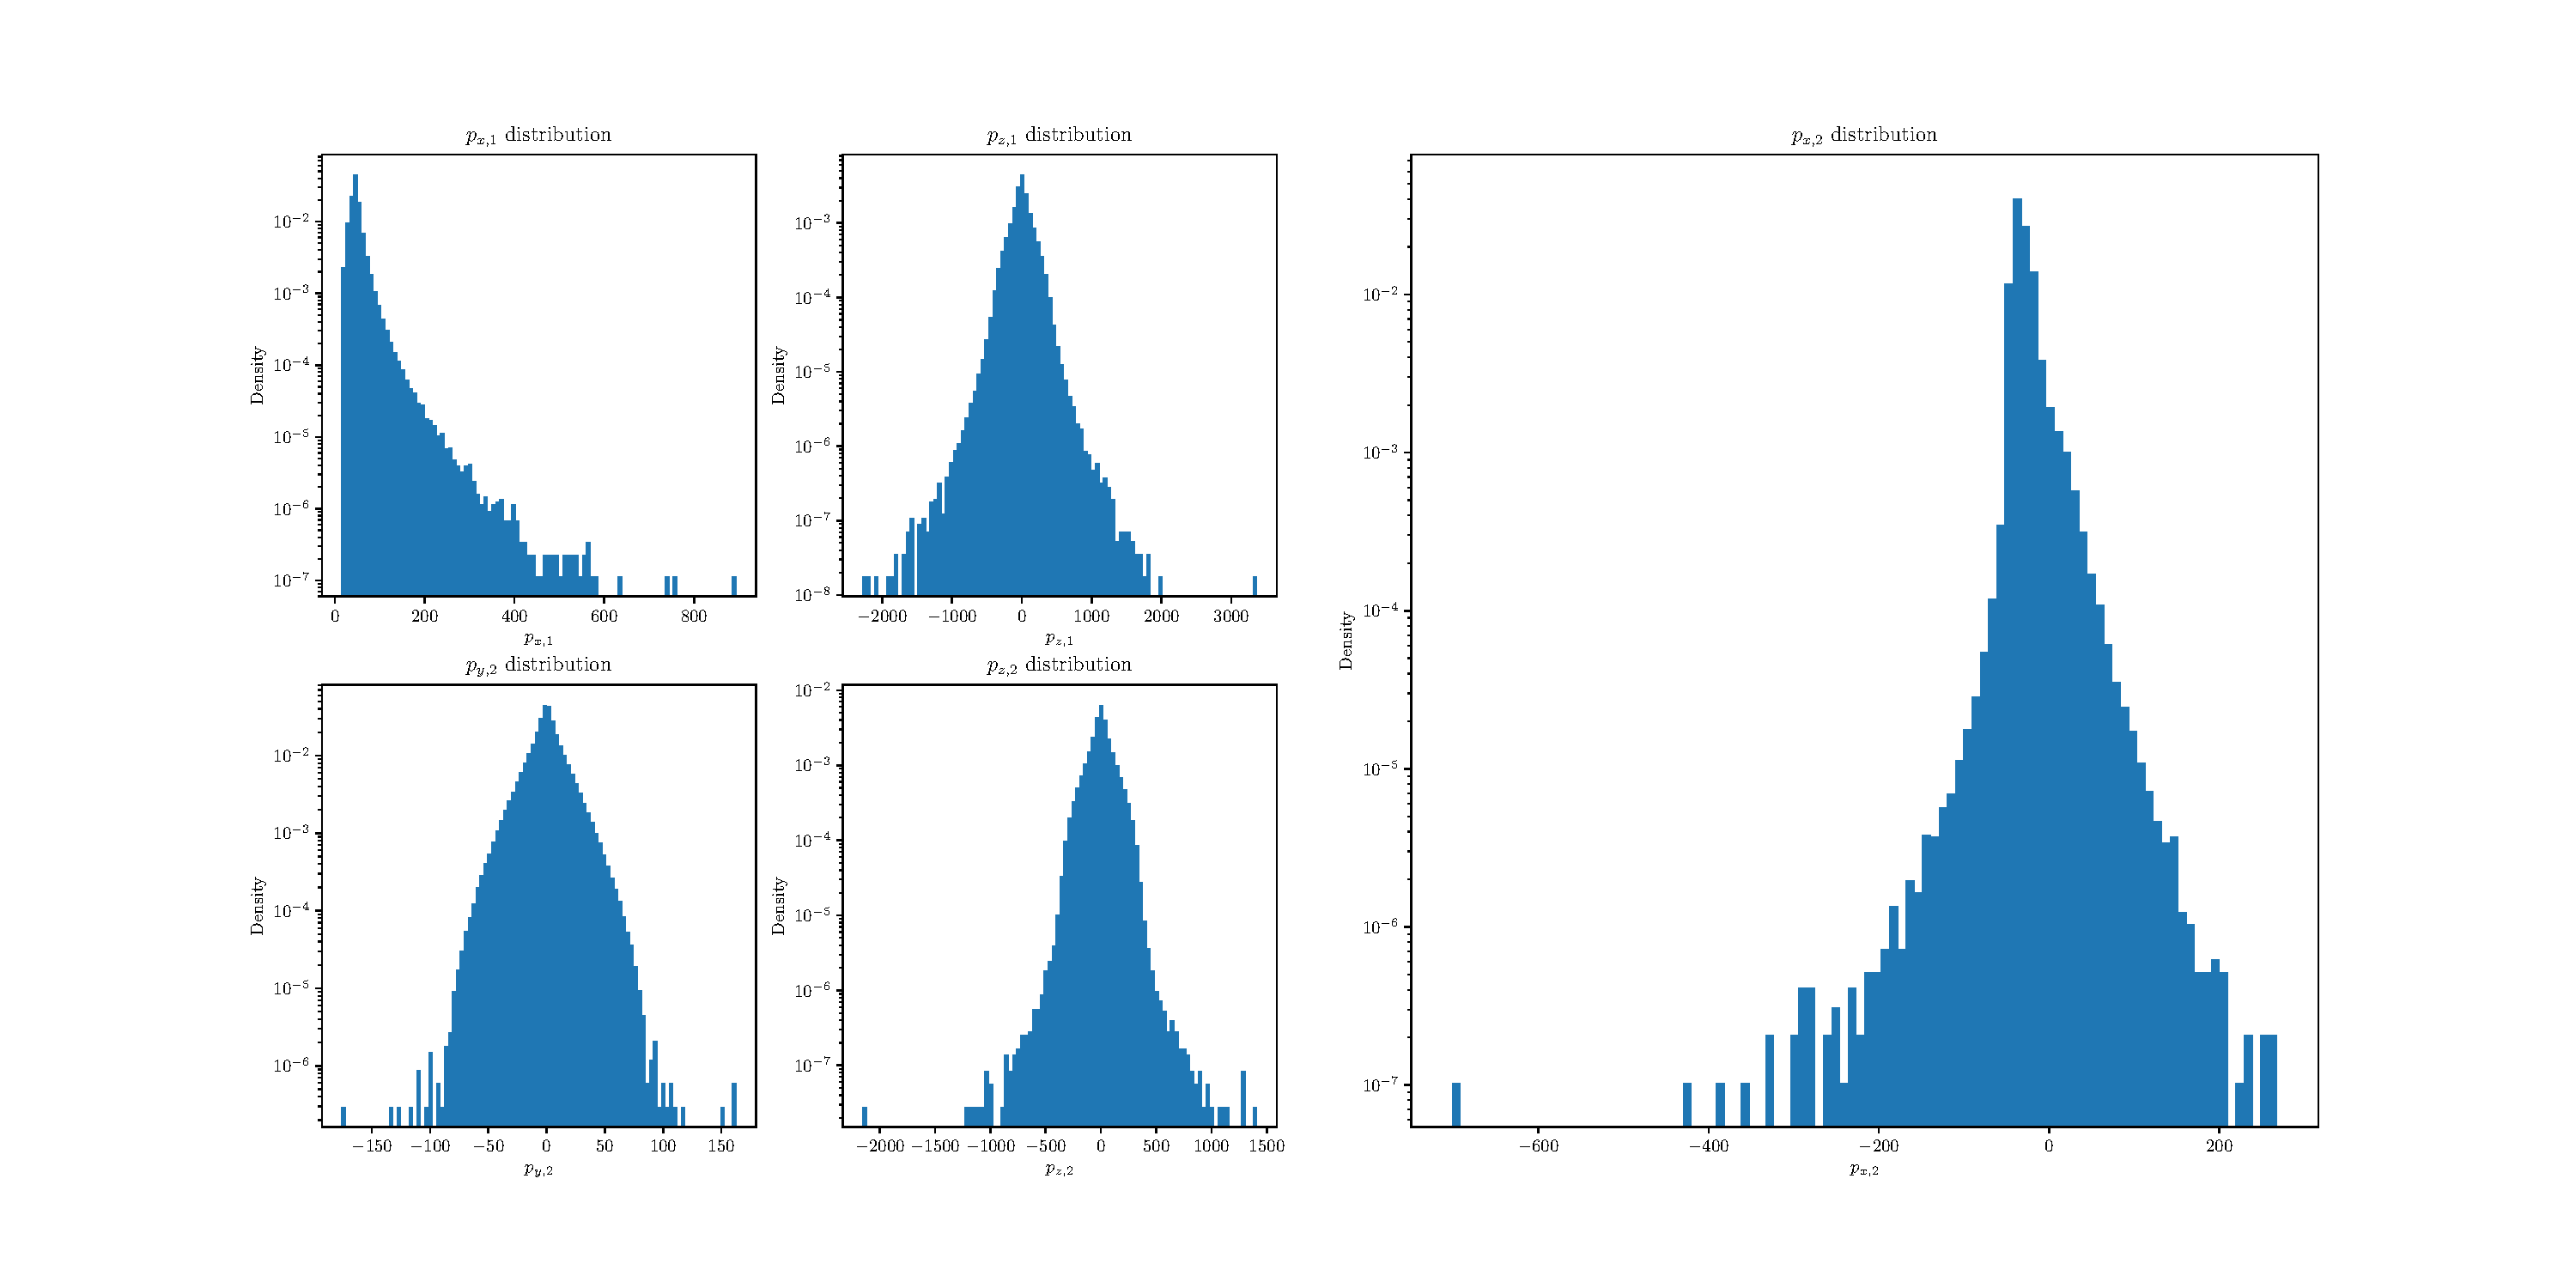
\includegraphics[width=1.0\textwidth]{Python/Z/data.pdf}
		\caption{Data distribution.}
		\label{fig:DATA_DISTRIBUTIONS}
	\end{center}
\end{figure}

\begin{figure}[H]
	\begin{center}
		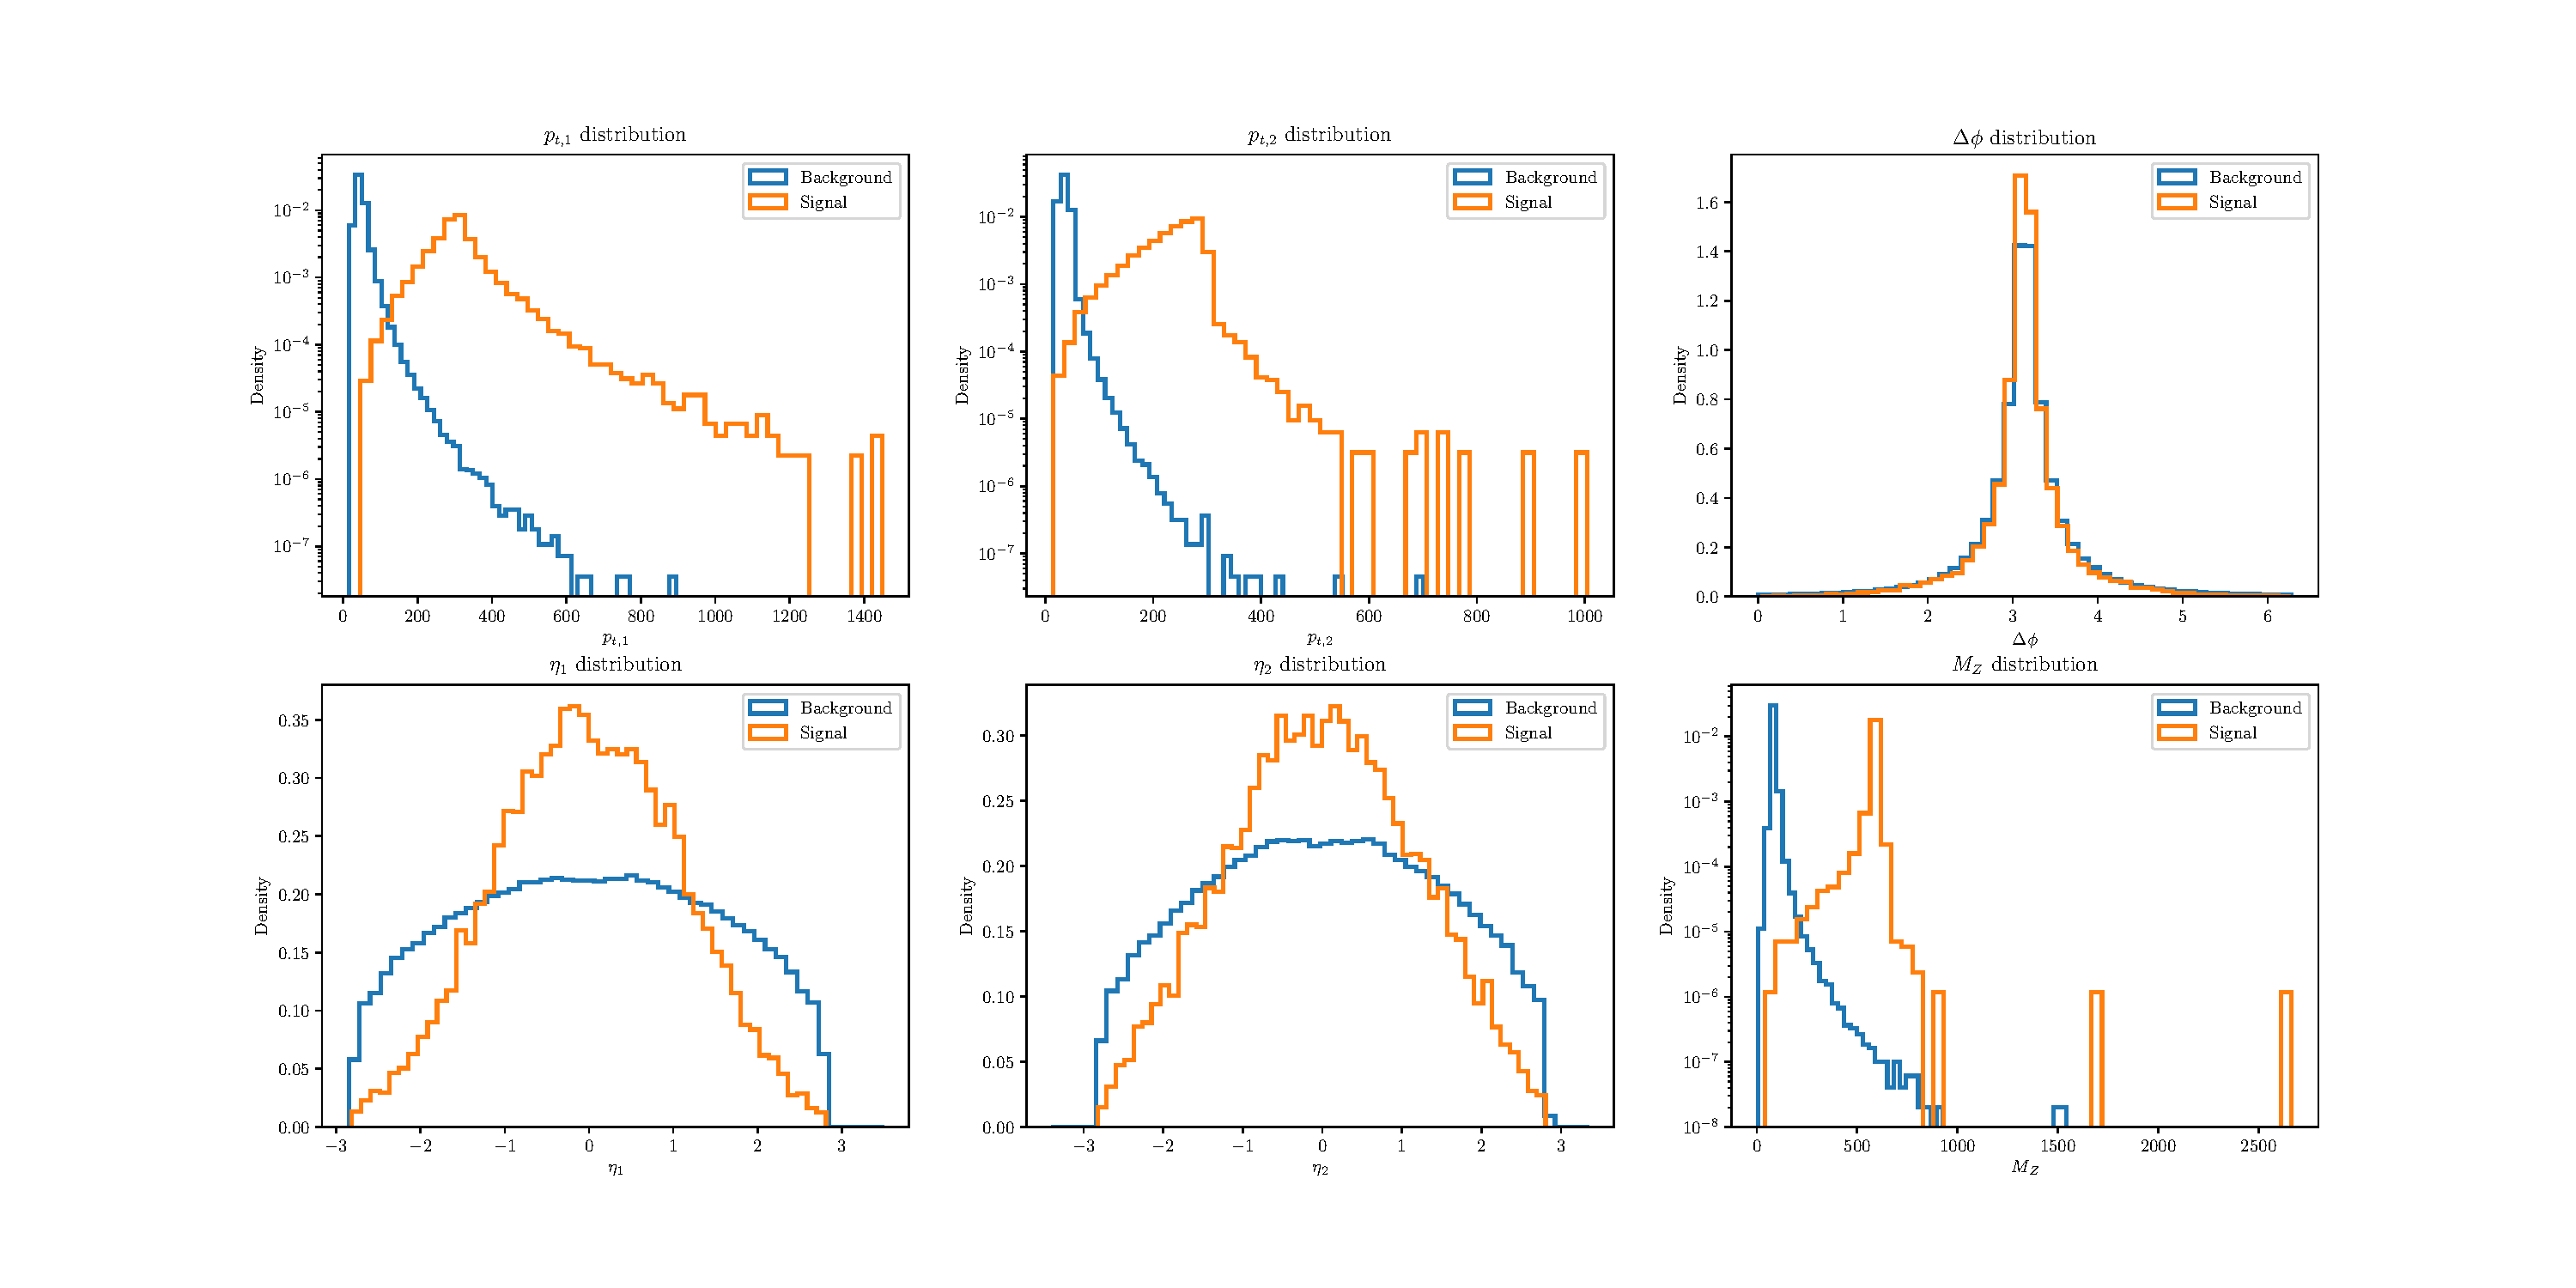
\includegraphics[width=1.0\textwidth]{Python/Z/features.pdf}
		\caption{Features and invariant mass distributions.}
		\label{fig:FEATURES_DISTRIBUTIONS}
	\end{center}
\end{figure}

\begin{figure}[H]
	\begin{center}
		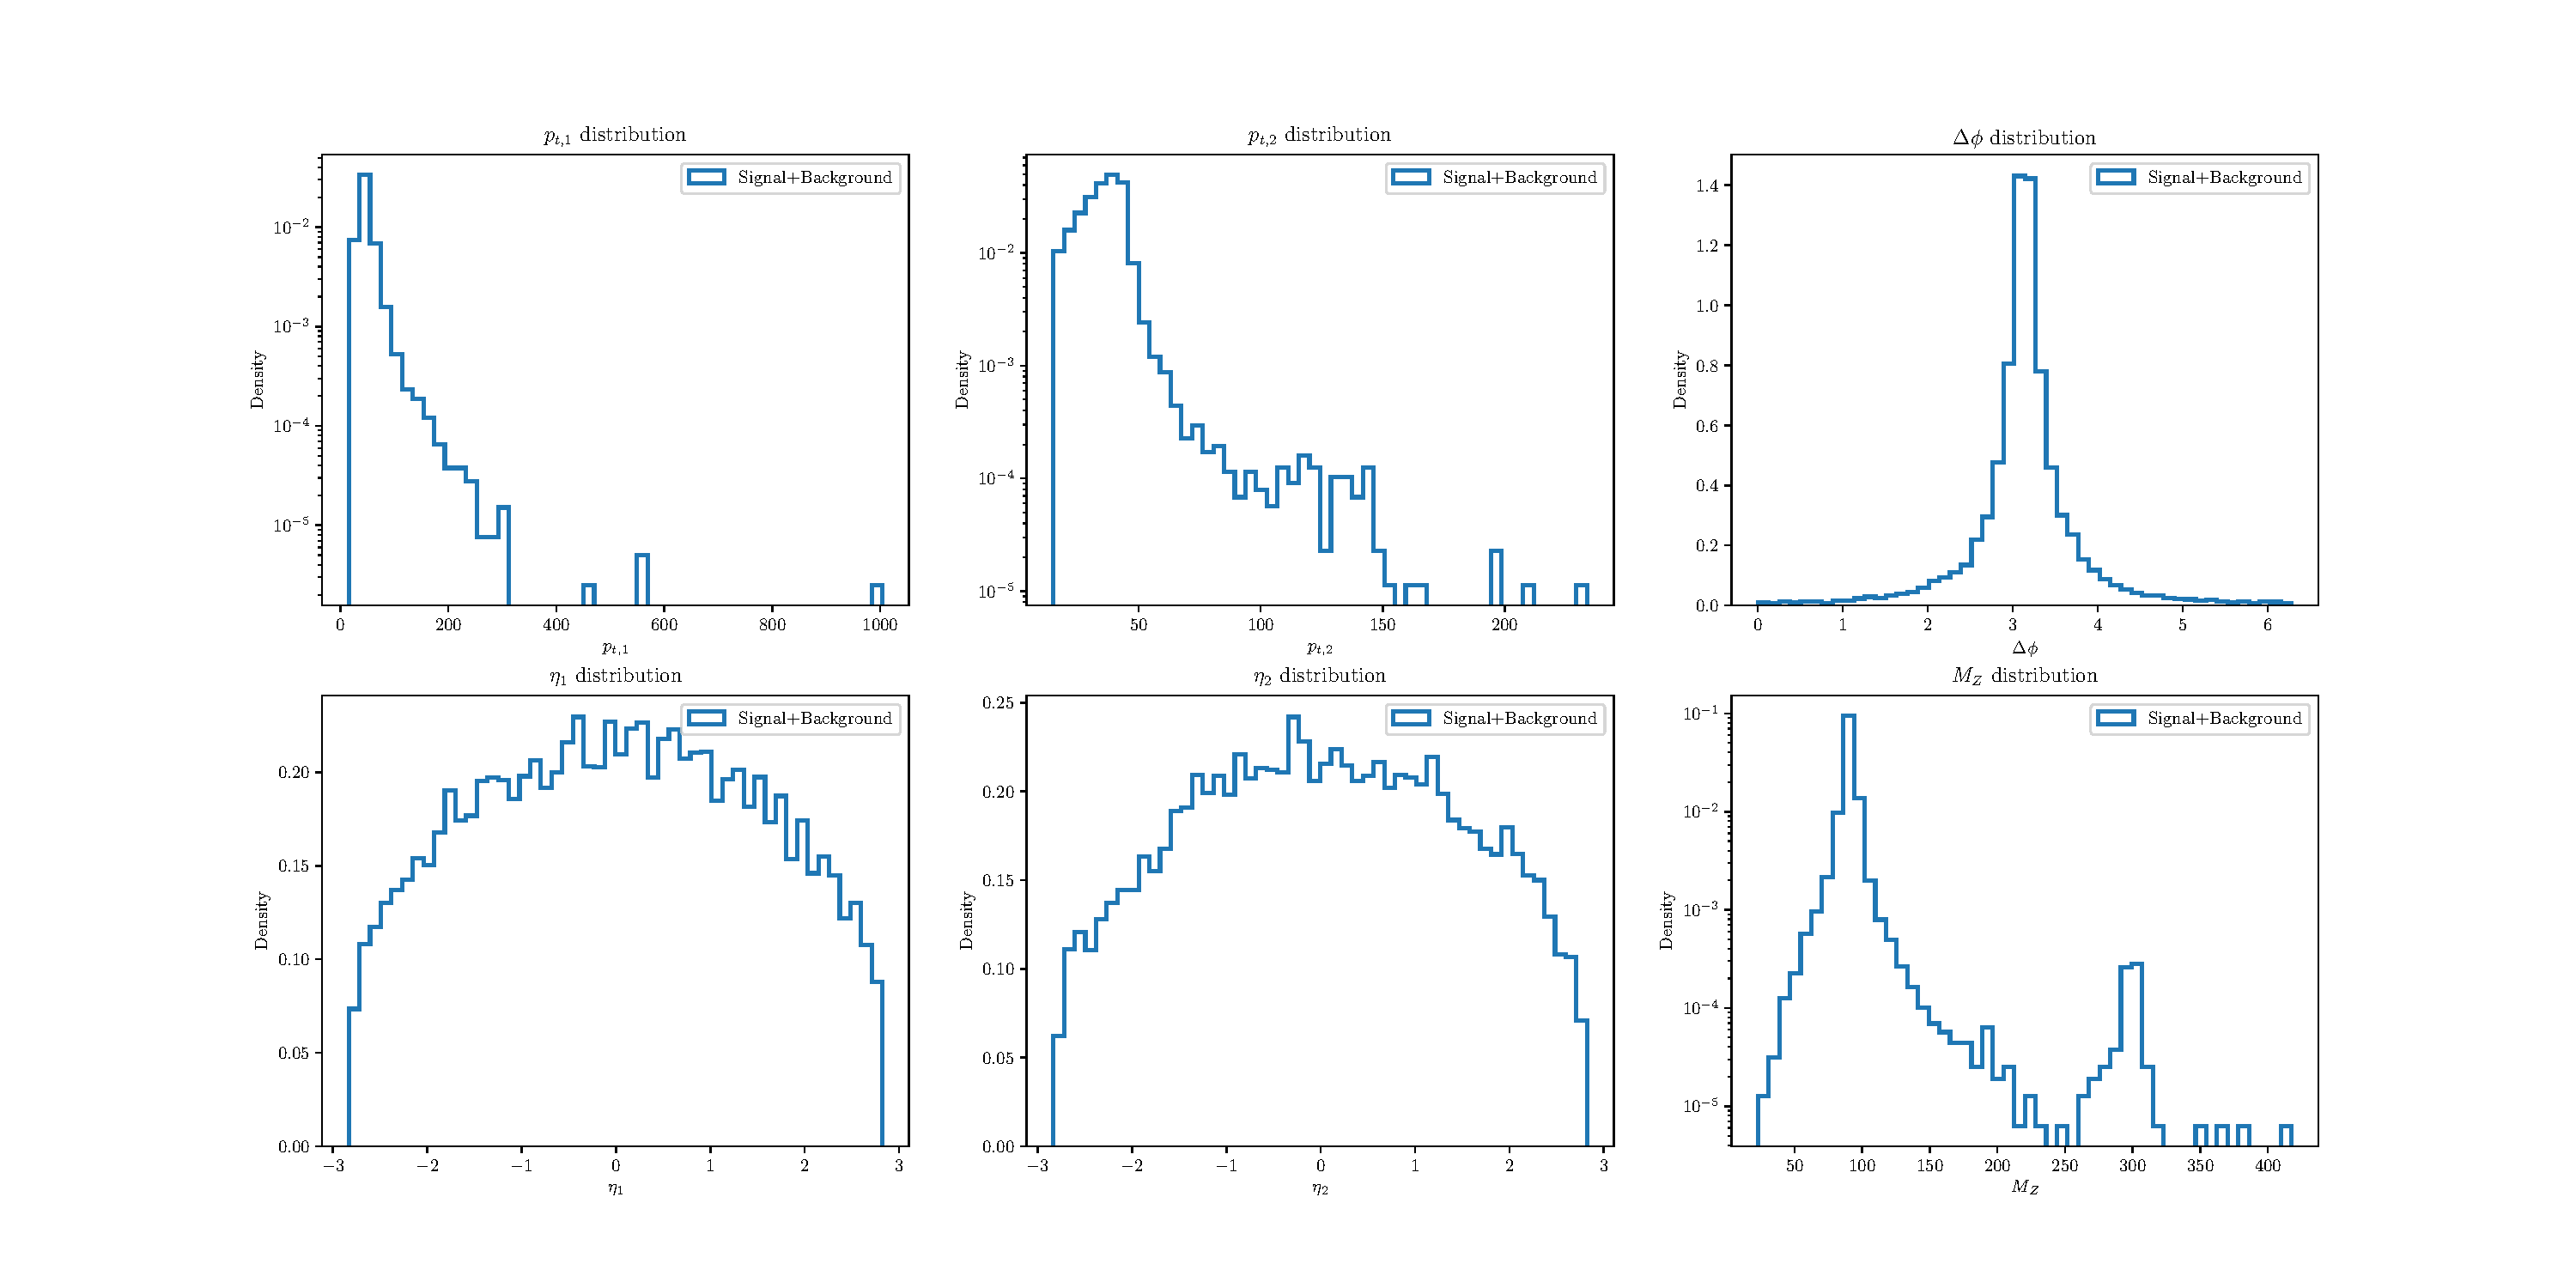
\includegraphics[width=1.0\textwidth]{Python/Z/sig_plus_bkg.pdf}
		\caption{Features and invariant mass distributions with signal+background in the same dataset.}
		\label{fig:SIG_PLUS_BKG_DISTRIBUTIONS}
	\end{center}
\end{figure}